\documentclass[tikz,border=2pt]{standalone}
\usepackage{amsmath,amssymb}
\usepackage{tikz}
\usetikzlibrary{arrows.meta}

\begin{document}
% Polar form: a complex number is fixed by its modulus r = |z| and its argument phi.
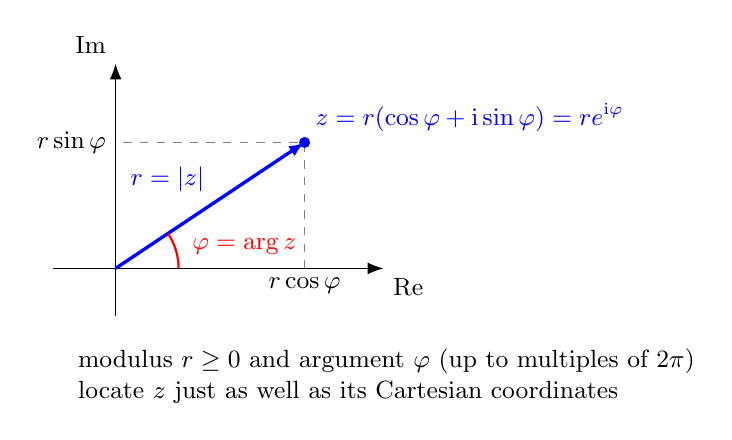
\begin{tikzpicture}[every node/.style={font=\small}, >={Latex[length=2mm]}]
	\draw[->] (-0.8,0) -- (3.4,0) node[below right] {$\mathrm{Re}$};
	\draw[->] (0,-0.6) -- (0,2.6) node[above left] {$\mathrm{Im}$};
	\draw[dashed, gray] (2.4,0) -- (2.4,1.6) -- (0,1.6);
	\draw[->, blue, very thick] (0,0) -- (2.4,1.6) node[above right] {$z=r(\cos\varphi+\mathrm{i}\sin\varphi)=re^{\mathrm{i}\varphi}$};
	\fill[blue] (2.4,1.6) circle (2pt);
	\node[blue, above left] at (1.25,0.85) {$r=|z|$};
	\draw[red, thick] (0.8,0) arc (0:33.7:0.8);
	\node[red, right] at (0.85,0.28) {$\varphi=\arg z$};
	\node[below, font=\small] at (2.4,0) {$r\cos\varphi$};
	\node[left, font=\small] at (0,1.6) {$r\sin\varphi$};
	\node[anchor=north west, align=left] at (-0.6,-0.9) {modulus $r\ge0$ and argument $\varphi$ (up to multiples of $2\pi$)\\ locate $z$ just as well as its Cartesian coordinates};
\end{tikzpicture}
\end{document}
